\documentclass[doktyp=parbeit]{TUBAFarbeiten}

\usepackage{selinput}% Auswahl der Dateikodierung (ansi,latin1,utf8,...)
\SelectInputMappings{adieresis={ä},germandbls={ß},Euro={€}}% Zeichenzuordnung für selinput.sty
%\usepackage[T1]{fontenc}% Einstellung Fontencoding
%\usepackage[utf8]{inputenc}
\usepackage{lmodern}
\usepackage{csquotes}% Einstellung zu Anführungszeichen; wird von biblatex.sty gefordert
\usepackage[backend=biber,style=numeric-comp,sorting=none]{biblatex}% bessere Literaturverarbeitung
\addbibresource{Literatur.bib}% welche Literaturdatenbank genutzt werden soll; Endung nicht vergessen!
\ExecuteBibliographyOptions{
	bibwarn=true, %Probleme mit den Daten, die Backend betreffen anzeigen
	isbn=false, %keine isbn anzeigen
	doi=true,
	url=false
}

\usepackage{booktabs}							% bessere Tabellenformatierung
\usepackage{amsmath}							% mehr Mathe
\usepackage{tabularx}							% Tabellen auf Textbreite ausdehnen
\usepackage{float}						       	% H-Paramter für floats
\usepackage{lscape}
\usepackage{icomma}
\usepackage{amsfonts}
\usepackage{subfiles}
\usepackage{mathtools,amssymb}
\usepackage{graphicx}
\usepackage[version=3,arrows=pgf]{mhchem}				% Chemie: Summenformeln
\usepackage{siunitx}[2010/05/23]					% Einheiten formatieren
\sisetup{per-mode=symbol}
\DeclareSIUnit\sq{\ensuremath{\Box}}
\sisetup{%
	detect-all,				% alle äußeren Schrifkonventionen übernehmen
	per-mode=fraction,		% \per erzeugt Bruch
	output-decimal-marker={,},	% Dezimaltrennzeichen ist Komma
	unit-mode=text			% Einheiten im Textmodus
}
\hbadness=10000
\vbadness=10000
\usepackage[colorlinks,
pdfpagelabels,
pdfstartview = FitH,
bookmarksopen = true,
bookmarksnumbered = true,
linkcolor = black,
plainpages = false,
hypertexnames = false,
citecolor = black] {hyperref}
\usepackage{listings}
\usepackage{color}

\definecolor{dkgreen}{rgb}{0,0.6,0}
\definecolor{gray}{rgb}{0.5,0.5,0.5}
\definecolor{mauve}{rgb}{0.58,0,0.82}
\lstset{frame=tb,
	language=Java,
	aboveskip=3mm,
	belowskip=3mm,
	showstringspaces=false,
	columns=flexible,
	basicstyle={\small\ttfamily},
	numbers=none,
	numberstyle=\tiny\color{gray},
	keywordstyle=\color{blue},
	commentstyle=\color{dkgreen},
	stringstyle=\color{mauve},
	breaklines=true,
	breakatwhitespace=true,
	tabsize=3
}

%\usepackage{setspace}% Einstellungen Zeilenabstand
%\onehalfspacing% Einstellungen Zeilenabstand

%\TUBAFFakultaet{Fakultät für Biotechnologie und Ökologie}
%\TUBAFInstitut{Institut für Agrarindustrie}
%\TUBAFLehrstuhl{Lehrstuhl für Bodenkultur}

%\TUBAFZweitlogo{\includegraphics{thekla_logo.jpg}}

\TUBAFTitel{Nutzerdokumentation\\ML.NET-Bildklassifzierung}%
\TUBAFUntertitel{Konsolenanwendung}
%\TUBAFBetreuer{Prof.\,Dr.\,rer.nat. Yvonne Joseph}
%\TUBAFKorrektor{Korrektor zwei}
\TUBAFAutor[A. Kaufmann/R. Mende]{Alexander Kaufmann\\Robert Mende}
\TUBAFStudiengang{Nanotechnologie\\Chemie}
%\TUBAFVertiefung{Biotechnologie}
%\TUBAFMatrikel{63472}
\TUBAFDatum[2021-07-27]{27. Juli 2021}

\begin{document}
	
	\maketitle
	
	\tableofcontents
\section{Motivation}
Machine Learning stellt eine Möglichkeit dar, Computer analog zum menschlichen Lernen anhand von Erfahrungen lernen zu lassen. Dabei umfasst das Machine Learning ein weites Feld möglicher Anwendungsbereiche, wobei die Bildklassifizierung ein solches darstellt. Mit der vorliegenden Software können Bilder mittels eines zuvor in der Software trainierten Modells klassifiziert werden. 
Zum Einsatz kommt dazu ein von Google erstelltes neuronales Netz „Inception v1“ nach dem Vorbild des \href{https://docs.microsoft.com/de-de/dotnet/machine-learning/tutorials/image-classification}{Dokumentationsbeispieles} von ML.Net.
\section{Anwendungsfeld der Software}
Die Software kann prinzipiell zur Kategorisierung von Bildern der Typen .jpg und .png verwendet werden. Die Verwendung der mit der Software erzeugten Vorhersagemodelle ist jedoch nur mit ungelabelten Bildern sinnvoll, die tatsächlich zu einem der vorher trainierten Labels gehören. Dementsprechend führen beispielsweise Bilder von Fahrzeugen bei einem Modell, das zur Klassifizierung verschiedener Blumen trainiert wurde, zu willkürlichen Zuweisungen.
Im Gegenzug kann die Software je nach Größe der Trainingsdaten, Unterschiedlichkeit zwischen den trainierten Labels etc. durchaus zuverlässig neue Bilder klassifizieren. 
Weiterhin kann das Modell vom Nutzer auf neue Kategorien trainiert werden. Dazu kommt das Neurale Netz \texttt{InceptionV1} von Google zum Einsatz. Die notwendigen Bilder werden aus der freien Datenbank \href{https://storage.googleapis.com/openimages/web/index.html}{Open Images Dataset V6} heruntergeladen. Auf Basis eines neu trainierten Modells kann die Bildklassifikation wieder aufgerufen werden.
\section{Benutzung der Software}
\subsection{Vorbereitungen}
\subsubsection{Releasebuild}
\subsubsection*{Runtime}
Die Software wurde für \texttt{.NET 5.0} geschrieben. Zu Ausführung ist die entsprechende \href{https://dotnet.microsoft.com/download}{Runtime} notwendig.
\subsubsection*{Zusätzliche Dateien}
Zum Trainieren neuer Modelle können Bilder aus einem AWS Bucket heruntergeladen werden. Der \href{https://storage.googleapis.com/openimages/v6/oidv6-train-annotations-human-imagelabels.csv}{Datenbankindex} ist jedoch zu groß für Github und muss separat von Hand heruntergeladen werden. Datei besitzt eine Größe von ca. 2,5 Gb. Nach dem Herunterladen muss die Datei auf eine Ebene mit der \texttt{.Index}-Datei kopiert werden und in \texttt{imageIDs.csv} umbenannt werden. Die Ordnerstruktur sollte Abb. \ref{fig:release} entsprechen. Das Programm ist nun einsatzbereit.
\begin{figure}
	\centering
	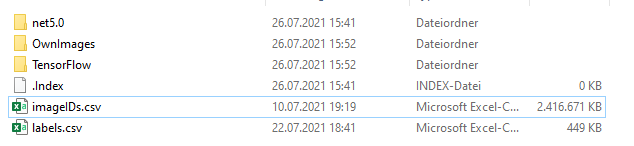
\includegraphics[width=0.7\linewidth]{Bilder/Release}
	\caption{Ordnerstruktur für den Release-Build}
	\label{fig:release}
\end{figure}
\subsubsection{Build von Sourcecode}
Die Quellcode ist über Github download verfügbar und kann über die \texttt{.Net-SDK} kompiliert werden. Die zusätzliche \texttt{.csv}-Datei ist analog dem Releasebuild herunterzuladen und auf einer Ebene mit der \texttt{.Index}-Datei zu speichern. Das Programm kann durch das erstellen eines Builds der \texttt{ConsoleApp} gestartet werden. Die Ordnerstruktur sollte Abb. \ref{fig:github} entsprechen. Wenn der Ordner \texttt{TensorFlow} fehlt, muss dieser von Hand erstellt werden und das \href{https://storage.googleapis.com/download.tensorflow.org/models/inception5h.zip}{neuronale Netz} von Hand direkt dort eingefügt werden (\texttt{.pb-Datei}). Sollte die vorhandene \texttt{tensorflow\_inception\_graph.pb}-Datei im Ordner \texttt{TensorFlow} korumpiert sein, befindet sich im \texttt{zip}-Verzeichnis \texttt{inception5h.bac} ein Backup.
\begin{figure}
	\centering
	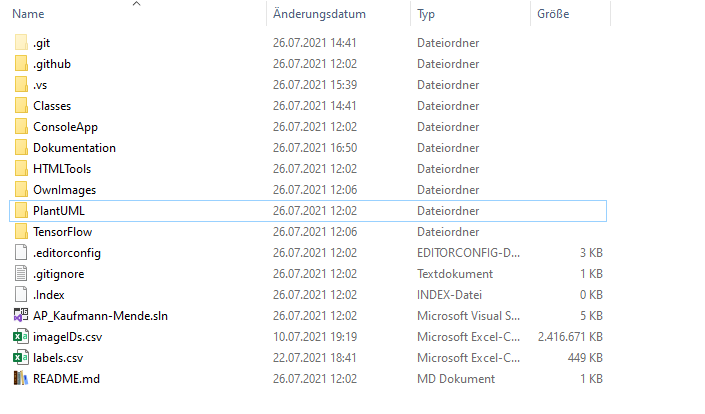
\includegraphics[width=0.7\linewidth]{Bilder/github}
	\caption{Ordnerstruktur des Projektes, fertig zum kompilieren}
	\label{fig:github}
\end{figure}
\subsubsection*{NuGet-Packages}
Sämtliche benötigten NuGet-Packages werden in der Solution- bzw. Projekt-Datei vermerkt. Die benötigten Pakete müssen im Paketmanager mit \texttt{nuget restore AP\_Kaufmann-Mende.sln} wieder hergestellt werden, \textbf{sollten sie nicht automatisch durch NuGeT heruntergeladen werden}. Achtung: es werden ca. \textbf{2 Gb} des in der \texttt{.NET-SDK} hinterlegten Nutzerverzeichnisses zusätzlich belegt. Hiermit sind die Vorbereitungen abgeschlossen.	
\section{Nutzung der Software}
\subsection{Benutzeroberfläche}
Ausgeführt wird eine Konsolenapp in \texttt{.NET 5}, die dem Nutzer nach Start der Software zwei Möglichkeiten bietet: 
\begin{itemize}
	\item Das Training eines Modells, um nachfolgend damit Bilder klassifizieren zu können
	\item Die Klassifizierung von Bildern, die sich in einem vorgegebenen Ordner befinden
\end{itemize}
Die Entscheidung ist anhand der Eingabe der Taste 1 beziehungsweise 2 unmittelbar nach dem Start zu treffen. 
\subsubsection{Auswahl des Trainingsmodus}
Der Trainingsmodus dient programmintern zur Erstellung eines Modells, das Bilder im vom Nutzer vorgegebene Kategorien einteilt. Dementsprechend wird der Nutzer nach Eintritt in den Trainingsmodus aufgefordert, einen Suchbegriff vorzugeben. Anhand dieses Begriffes wird in der Datenbank nach Labels gesucht, die den vorgegebenen Begriff enthalten. Diese Labels werden dem Nutzer anschließend zum Training vorgeschlagen. 

Der Nutzer wählt anschließend über die Eingabe einer oder mehrerer Zahlen diejenigen Labels, auf die er sein Modell trainieren möchte. An dieser Stelle ist die Interaktion des Nutzers mit dem Trainingsmodus abgeschlossen und das Modell wird trainiert. Die Bilder werden zuvor aus einem Amazon Cloud Storage (AWS Bucket) heruntergeladen. Je nach Umfang der Trainingsbilder kann dieser Vorgang viel Zeit in Anspruch nehmen.
\subsection{Auswahl des Klassifizierungsmodus}
Im Klassifizierungsmodus können anhand eines zuvor erstellten Modells Bilder aus dem Ordner \texttt{OwnImages}, der sich im gleichen Ordner wie die \texttt{.Index} oder die \texttt{AP\_Kaufmann-Mende.sln}-Datei befindet, geladen und klassifiziert werden. Die Bilder sollten dabei im \texttt{.jpg}- oder \texttt{.png}-Format vorliegen. 

Wird der Klassifizierungsmodus im Hauptmenü durch Drücken der Taste 1 ausgewählt, so werden alle indizierten, zuvor trainierten Modelle angezeigt. Über Eingabe von deren Index und die Bestätigung mit Enter kann nun ein einzelnes Modell geladen werden. Dieses Modell wird anschließend genutzt, um die im \texttt{OwnImages}-Ordner liegenden Bilder zu klassifizieren. 

Die Ausgabe der vorhergesagten Labels erfolgt anhand einer \texttt{HTML}-Datei im Ordner \texttt{OwnImages}. In der \texttt{HTML}-Datei befinden sich die Label, welche Verlinkungen auf die jeweiligen Bilder besitzen.
%	\printbibliography[heading=bibintoc]
	%\TUBAFErklaerungsseite
\section{Abbruchkriterien}
Im Falle verschiedener Fehler wird das Programm beendet:
\subsubsection*{Kategorisierung eigener Bilder}
\begin{itemize}
	\item Kein trainiertes Modell vorhanden
\end{itemize}
\subsubsection*{Trainieren eigener Modelle}	
\begin{itemize}
	\item \texttt{csv}-Dateien nicht vorhanden oder der Header der \texttt{csv}-Dateien ist falsch
	\item keine Verbindung zu Amazon-Diensten möglich
	\item Tensorflow-Inception-Neural-Network nicht vorhanden
\end{itemize}
Außerdem bricht das Programm ab, wenn nur unzureichende Schreib-/Leserechte vorliegen.  
\section{Known Issues}
Die Download-API von AWS friert teilweise das Programm ein, in dem Falle muss das Programm neugestartet werden. Leider konnten dazu keine weiteren Information gefunden werden. 
\section{Umsetzung}
Die Programmierung erfolgte von Alexander Kaufmann und Robert Mende. Die Grundstruktur des Training des Tensorflow-Abschnittes stammt aus \href{https://docs.microsoft.com/de-de/dotnet/machine-learning/tutorials/image-classification}{Dokumentationsbeispiel} von ML.Net. Die einzelnen Funktionen sind mittels der integrierten XML-Dokumentation von Visual Studio kommentiert.  
\section{Links}
\begin{itemize}
	\item Dokumentationsbeispiel ML.Net Bildklassifizierung: \url{https://docs.microsoft.com/de-de/dotnet/machine-learning/tutorials/image-classification}
	\item Open Images Dataset V6 \url{https://storage.googleapis.com/openimages/web/index.html}
	\item Microsoft \texttt{.Net} \url{https://dotnet.microsoft.com/download}
	\item Image-IDs der Open Images Dataset V6-Datenbank \url{https://storage.googleapis.com/openimages/v6/oidv6-train-annotations-human-imagelabels.csv}
	\item neuronales Netz Inceptionv1 \url{https://storage.googleapis.com/download.tensorflow.org/models/inception5h.zip}
\end{itemize}
\addsec{Anhang}
\begin{landscape}
	\begin{figure}
		\centering
		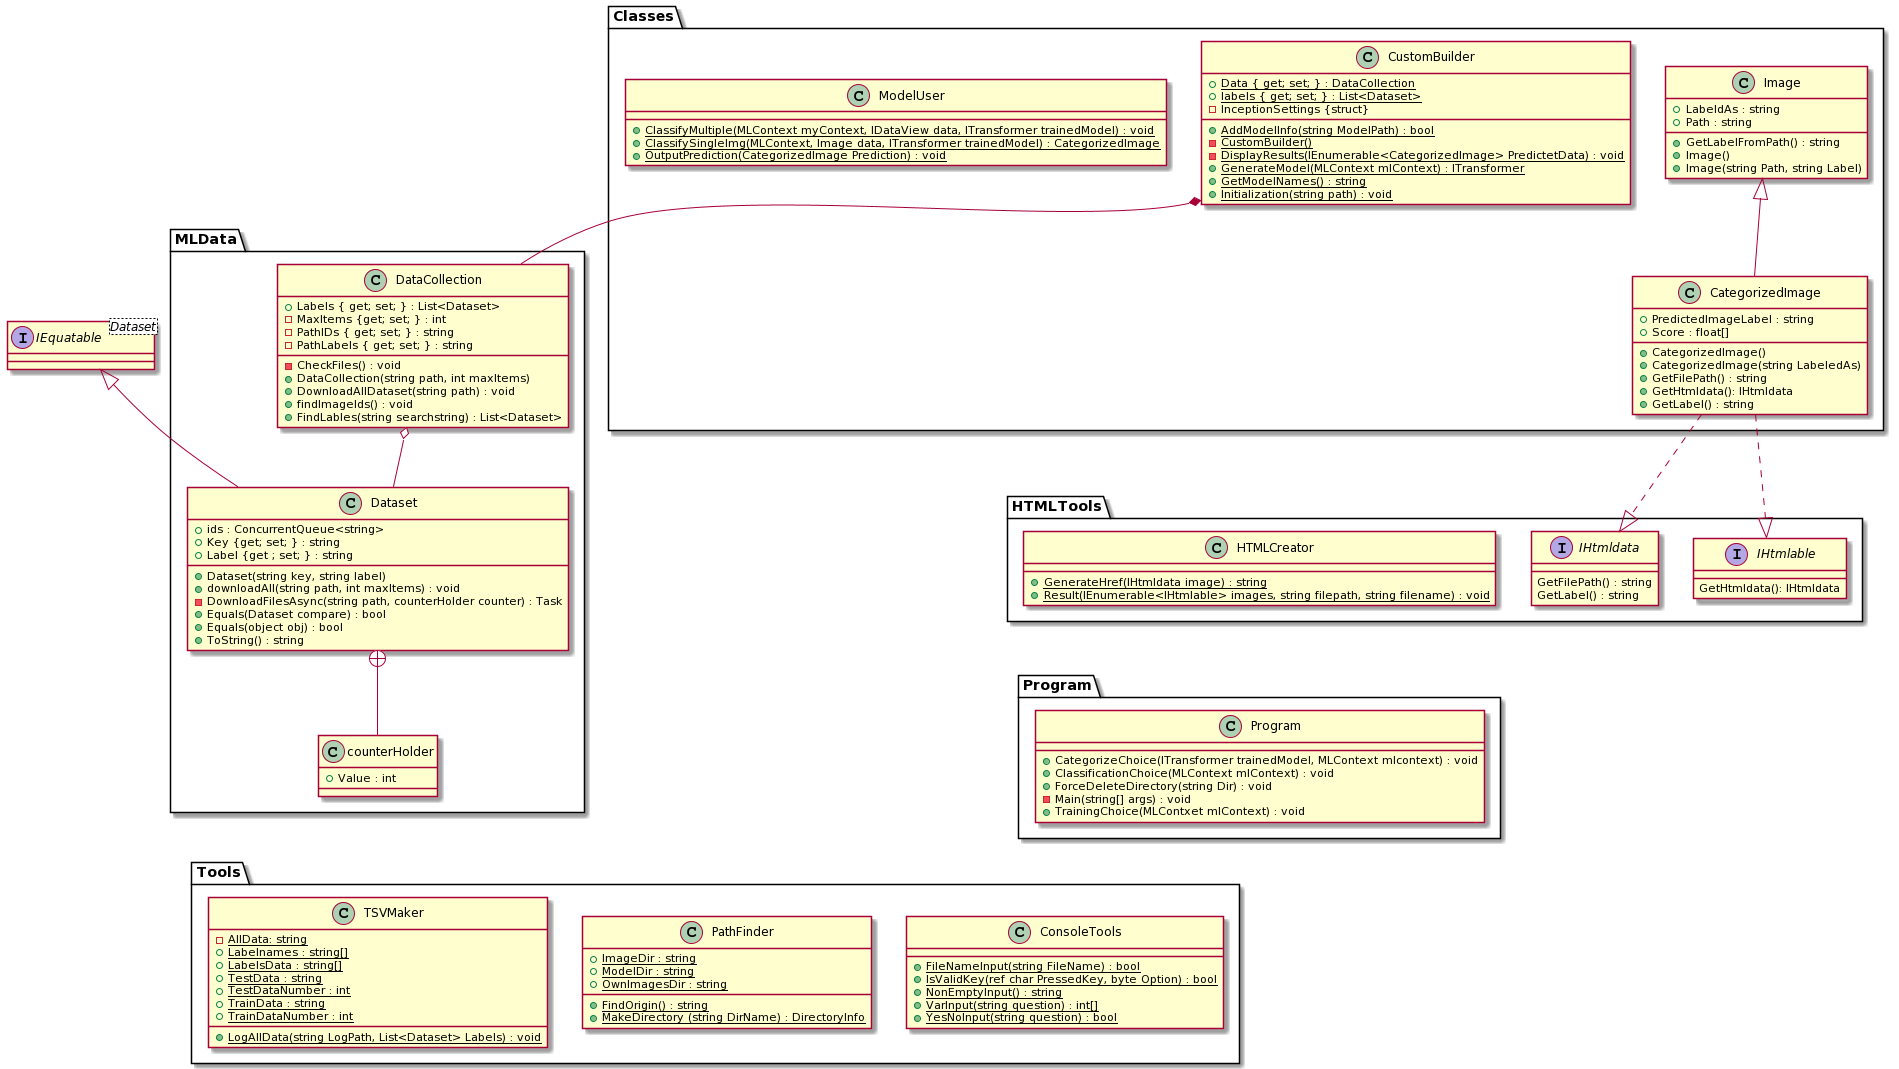
\includegraphics[width=1\linewidth]{Bilder/Classdiagramm}
		\caption{Klassendiagramm des finalen Programms}
		\label{fig:classdiagramm}
	\end{figure}
	
\end{landscape}
\end{document}